% Snowflake Data Engineering — Chapter 9 | original manuscript draft
% Author: Arman Golbidi | Editorial snapshot: 22 October 2026
% Compile: xelatex -interaction=nonstopmode -halt-on-error Snowflake_Data_Engineering_Chapter_08.tex
% Trim: 178 x 254 mm; margins inside 23 mm / outside 17 mm / top-bottom 19 mm.
% Body: 10.75 pt / 13.65 pt leading = 1.27 line-height ratio; code: 8.75 pt.
\documentclass[11pt,twoside]{article}
\usepackage[paperwidth=178mm,paperheight=254mm,inner=23mm,outer=17mm,top=19mm,bottom=19mm,headheight=5mm,headsep=4mm,footskip=9mm]{geometry}
\usepackage{fontspec}
\setmainfont{LibertinusSerif-Regular.otf}[BoldFont=LibertinusSerif-Bold.otf,ItalicFont=LibertinusSerif-Italic.otf,BoldItalicFont=LibertinusSerif-BoldItalic.otf]
\setsansfont{LibertinusSans-Regular.otf}[BoldFont=LibertinusSans-Bold.otf,ItalicFont=LibertinusSans-Italic.otf]
\setmonofont{LibertinusMono-Regular.otf}[Scale=0.91]
\usepackage[english]{babel}
\usepackage{microtype}
\usepackage{setspace}
\setstretch{1.0}
\usepackage{titlesec,enumitem,tabularx,array,booktabs,needspace,fancyhdr,lastpage}
\usepackage[most]{tcolorbox}
\usepackage{tikz}
\usetikzlibrary{arrows.meta,positioning,fit,shapes.misc,calc}
\usepackage{listings}
\usepackage{xcolor}
\usepackage{hyperref}
\usepackage{amsmath}
\hypersetup{colorlinks=true,urlcolor=steelblue,linkcolor=steelblue,pdfauthor={Arman Golbidi},pdftitle={Snowflake Data Engineering - Chapter 9: Data Engineering with Snowpark Python},pdfsubject={English technical book manuscript, ninth chapter, 178 x 254 mm}}
\definecolor{navy}{HTML}{15334A}
\definecolor{steelblue}{HTML}{17779B}
\definecolor{teal}{HTML}{12888A}
\definecolor{lightblue}{HTML}{ECF5F7}
\definecolor{papergray}{HTML}{F2F5F6}
\definecolor{inkgray}{HTML}{4A5862}
\definecolor{thinrule}{HTML}{CBD7DB}
\AtBeginDocument{\color{navy}\fontsize{10.75}{13.65}\selectfont}
\setlength{\parindent}{0pt}
\emergencystretch=2.5em
\setlength{\parskip}{3.3pt plus 0.7pt minus 0.6pt}
\setlist[itemize]{leftmargin=4mm,itemsep=1pt,topsep=2pt,parsep=0pt}
\setlist[enumerate]{leftmargin=5mm,itemsep=1pt,topsep=2pt}
\titleformat{\section}{\sffamily\bfseries\color{navy}\fontsize{14}{17}\selectfont}{}{0pt}{}
\titlespacing*{\section}{0pt}{8pt}{4pt}
\titleformat{\subsection}{\sffamily\bfseries\color{steelblue}\fontsize{10.8}{13}\selectfont}{}{0pt}{}
\titlespacing*{\subsection}{0pt}{5pt}{1pt}
\newcommand{\topic}[2]{\subsection*{#1\quad #2}}
\newcommand{\repo}[2]{\par\begingroup\fontsize{8.0}{9.6}\selectfont\sffamily\color{inkgray}\textbf{Project reference:} \href{#2}{#1}. \textit{Not independently executed; rights review pending.}\par\endgroup}
\newtcolorbox{insight}[1][]{enhanced,breakable,colback=lightblue,colframe=thinrule,boxrule=.45pt,arc=1.3mm,left=2.8mm,right=2.8mm,top=1.8mm,bottom=1.8mm,before skip=5pt,after skip=5pt,#1}
\newtcolorbox{whitebox}[1][]{enhanced,breakable,colback=papergray,colframe=thinrule,boxrule=.35pt,arc=1mm,left=2.6mm,right=2.6mm,top=1.5mm,bottom=1.5mm,before skip=4pt,after skip=5pt,#1}
\lstdefinestyle{chaptercode}{basicstyle=\ttfamily\fontsize{8.75}{10.7}\selectfont,backgroundcolor=\color{papergray},frame=single,framerule=.35pt,rulecolor=\color{thinrule},breaklines=true,columns=fullflexible,keepspaces=true,showstringspaces=false,aboveskip=5pt,belowskip=5pt,xleftmargin=2mm,xrightmargin=1mm,framexleftmargin=2mm,framexrightmargin=1mm}
\lstset{style=chaptercode}
\pagestyle{fancy}
\fancyhf{}
\fancyhead[LE]{\sffamily\fontsize{7.6}{9}\selectfont\color{inkgray}\textsc{Snowflake Data Engineering}}
\fancyhead[RO]{\sffamily\fontsize{7.6}{9}\selectfont\color{inkgray}\textsc{09 / Snowpark Python}}
\fancyfoot[LE,RO]{\sffamily\bfseries\fontsize{8.2}{9}\selectfont\color{steelblue}\thepage}
\fancyfoot[LO,RE]{\sffamily\fontsize{7.6}{9}\selectfont\color{inkgray}Arman Golbidi \quad | \quad Chapter 09}
\renewcommand{\headrulewidth}{0.35pt}
\renewcommand{\footrulewidth}{0pt}
\setcounter{page}{151}
\raggedbottom

% CHAPTER 08 ONLY, pages 133--150 in the planned book
% CHAPTER 09 ONLY: pages 151--170
\begin{document}
% PAGE 151 — opening
{\sffamily\bfseries\fontsize{9}{11}\selectfont\color{steelblue} CHAPTER 09 \hfill DATA ENGINEERING / SNOWPARK PYTHON}\par\vspace{3mm}
{\sffamily\bfseries\fontsize{21.2}{24.5}\selectfont\color{navy} Data Engineering with\\Snowpark Python}\par\vspace{2mm}
{\sffamily\fontsize{11.1}{14}\selectfont\color{steelblue} Write transformations in Python without losing the data platform}\par\vspace{4mm}
\begin{insight}\textbf{A correct transformation written in the wrong place can still be a bad design.}\par
The Finland Energy Analytics service receives a wind correction. The incoming event has a trusted business key and revision, but a junior engineer copies the entire bronze table to a laptop, filters the data in pandas, and uploads the result again. The calculation is right for six records. At national scale, the same pattern transfers sensitive rows across a trust boundary, creates an unbounded memory dependency, and makes retries harder to audit. There is a better question than ``Could Python express this calculation?'' It is ``Where should the calculation execute, and what proof of correctness survives deployment?''\end{insight}
Chapters~4--8 established data modelling, batch loading, JSON processing, delivery semantics and incremental state. Snowpark adds a \emph{Python interface to relational work} while preserving Snowflake's ability to execute supported operations near its data. It does not repeal the rules of secure access, deterministic business keys, idempotent updates or measured cost.
\begin{whitebox}\textbf{Learning outcomes}\par
After this chapter, you can (1) explain the difference between Python client orchestration and server-side execution; (2) manage least-privilege sessions; (3) build and inspect lazy DataFrame transformations; (4) evaluate joins, casts and aggregates; (5) decide between SQL, UDFs and stored procedures; (6) test without incurring cloud charges; and (7) design a maintainable, observable Snowpark pipeline.\end{whitebox}
\textbf{Prerequisites.} Chapters~3--6 and competent basic Python. SQL examples and production integration require access to a permitted Snowflake account. The bundled \emph{pure-Python offline fixture} runs on Python~3.10+ without network access; a Snowpark integration run is not claimed.
\begin{center}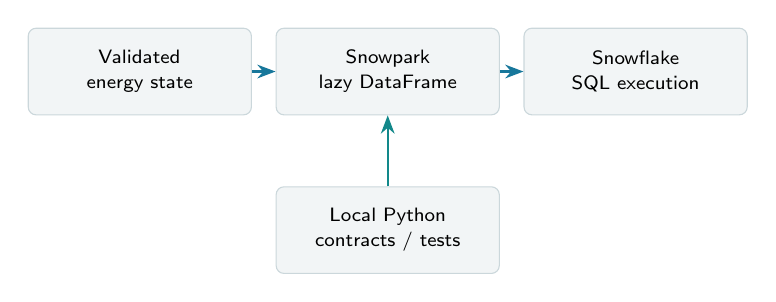
\begin{tikzpicture}[>=Stealth,every node/.style={font=\sffamily\fontsize{7.4}{9}\selectfont},n/.style={draw=thinrule,rounded corners=1mm,fill=papergray,align=center,text width=26mm,minimum height=11mm}]
\node[n](a){Validated\\energy state};\node[n,right=3mm of a](b){Snowpark\\lazy DataFrame};\node[n,right=3mm of b](c){Snowflake\\SQL execution};
\node[n,below=9mm of b](d){Local Python\\contracts / tests};
\draw[->,thick,steelblue](a)--(b);\draw[->,thick,steelblue](b)--(c);\draw[->,thick,teal](d)--(b);\end{tikzpicture}\\{\fontsize{8}{9.5}\selectfont\color{inkgray}Figure 9.1. Local control code defines a plan; supported relational work runs on Snowflake compute.}\end{center}
\newpage
% PAGE 152
\section*{9.1\quad Where Snowpark fits in the platform}
\topic{9.1.1}{Snowpark's role in data engineering}
Python has two distinct roles in an analytical platform: it can \emph{orchestrate} work and it can \emph{express} transformations. Snowpark provides a DataFrame API that lets Python code describe projections, filters, joins, windows and aggregations over Snowflake tables. For operations supported by the DataFrame API, the engine generates SQL and executes the relational plan in Snowflake. The Python process is not ordinarily reading every row to evaluate a \texttt{filter} expression itself. This division is both the central power of Snowpark and the source of many misconceptions.

Imagine an energy table with one approved row per provider, technology and UTC interval. To compute an hourly total, SQL is an excellent fit. A Snowpark DataFrame can express the same logic while sharing names, parameters and reusable business helpers with a broader Python codebase. The platform still performs the scan and aggregation. Snowpark is not a requirement to do analytics correctly; it is a reasonable interface when programmatic composition is valuable.
\begin{lstlisting}[language=Python,caption={Declarative query construction; cloud execution is not performed here.}]
from snowflake.snowpark.functions import col, sum as sf_sum
energy = session.table('ENERGY_SILVER')
plan = (energy.filter(col('ENERGY_MWH') >= 0)
        .group_by('INTERVAL_UTC')
        .agg(sf_sum('ENERGY_MWH').alias('TOTAL_MWH')))
# plan is a DataFrame, not a list of downloaded rows.
\end{lstlisting}
\textbf{Why it matters.} A transformation function can receive a session and return a DataFrame without writing a table, triggering data transfer, or choosing the consumer's schema. That separation makes a pipeline testable and lets an orchestrator own when an action should happen.
\begin{whitebox}\textbf{Architectural decision}\par
Use Snowpark when Python organisation, complex reusable expression-building, or Python runtime integration provides concrete value. If a small, stable SQL model already expresses the business rule transparently, introducing a Python application and dependencies may increase maintenance without improving correctness. Compare models against the same acceptance tests before introducing an extra runtime.\end{whitebox}
\repo{P094: Getting started with Snowpark Python}{https://github.com/Snowflake-Labs/sfguide-getting-started-snowpark-python}
\textbf{Check.} Is a DataFrame returned by \texttt{session.table()} an in-memory pandas DataFrame? Why does the distinction matter when a source table grows one hundredfold?
\newpage
% PAGE 153
\topic{9.1.2}{Python execution boundaries}
A Snowpark program crosses more than one boundary. The \emph{client} authenticates, creates a Session and constructs a logical DataFrame. \emph{Virtual warehouse compute} ordinarily executes supported query plans generated from that DataFrame. Python code inside a registered \emph{user-defined function} (UDF) or \emph{stored procedure} runs in a Snowflake-managed Python environment, subject to its applicable runtime and sandbox restrictions. These environments have different deployment, permissions and package availability; describing all three simply as ``Python runs in Snowflake'' obscures important operational detail.

\begin{center}\renewcommand{\arraystretch}{1.12}\begin{tabularx}{\linewidth}{@{}p{26mm}p{29mm}X@{}}\toprule
\textbf{Boundary}&\textbf{Typical action}&\textbf{Risk to control}\\\midrule
Client process&Construct DataFrame, call actions&Credential handling, accidental data collection\\
Snowflake SQL engine&Filter, join, aggregate&Compute consumption, scan volume, permissions\\
Python UDF/runtime&Execute Python handler&Package, sandbox, row processing overhead\\
External compute&Process exported data&Network exposure, duplication, transfer cost\\\bottomrule
\end{tabularx}\\{\fontsize{8}{9.5}\selectfont\color{inkgray}Table 9.1. Execution location determines data, security and cost obligations.}\end{center}
The code below \emph{looks} local, but the expensive relational operation belongs to a virtual warehouse when an action is called. Conversely, \texttt{collect()} returns a \emph{local list} and may materialise many rows in client memory. \texttt{to\_pandas()} similarly transfers a result to the Python process. Protect these actions with a narrow selection, a row limit for inspection, and explicit assertions about expected cardinality.
\begin{lstlisting}[language=Python,caption={Safe inspection versus unbounded client materialisation.}]
preview = plan.sort('INTERVAL_UTC').limit(5).collect()
# CAUTION: do not call plan.collect() on an unbounded dataset.
\end{lstlisting}
A Python worksheet in Snowsight, a notebook, a command-line application and a stored procedure may all use Snowpark, but their session ownership and deployment semantics differ. In a Python worksheet, the handler receives an existing session. A local command-line application normally constructs its own session. These examples must not be conflated when copied into production code.
\begin{insight}\textbf{Failure mode: hidden extraction}\par
An engineer writes a clean-looking function that calls \texttt{to\_pandas()}, then silently performs all grouping in local memory. Queries can appear fast in a six-row demonstration and later fail because the result is too large. Inspect the data movement as carefully as the formula.\end{insight}
\textbf{Check.} Which step transfers data: \texttt{group\_by(...)} or \texttt{collect()}?
\newpage
% PAGE 154
\topic{9.1.3}{Choosing SQL, Snowpark, or external compute}
A technology choice should be derived from the location of data, type of operation, governance boundary and operational ownership. SQL remains the clearest expression for many set-oriented joins, aggregations and window transformations. Snowpark is valuable when Python functions help assemble many consistent relational plans or when approved server-side Python algorithms are necessary. External compute is justified when a specialised library, runtime or integration cannot be deployed appropriately within Snowflake, but it increases the burden of moving data safely and proving reproducibility.
\begin{center}\renewcommand{\arraystretch}{1.09}\begin{tabularx}{\linewidth}{@{}p{26mm}X X@{}}\toprule
\textbf{Choice}&\textbf{Strong fit}&\textbf{Common downside}\\\midrule
SQL model&Stable declarative transformation&Complex Python control logic awkward\\
Snowpark DataFrame&Composed, reusable relational code&Additional Python dependency and tooling\\
Python UDF / procedure&Specialised logic near stored data&Runtime limits, packaging, row-level overhead\\
External Python&Custom integrations and runtimes&Extraction, network, identity, observability\\\bottomrule
\end{tabularx}\end{center}
\textbf{Example.} Convert unit-labelled synthetic meter readings to MWh with a simple expression. Writing this as an external Python loop would move data for no business reason. If the transformation instead requires a proprietary simulation package unavailable in the managed runtime, local or other cloud compute may be justified after a security and cost review.
\begin{lstlisting}[language=SQL,caption={A readable SQL baseline for equivalent Snowpark logic.}]
SELECT interval_utc, SUM(energy_mwh) AS total_mwh
FROM energy_silver
WHERE operation = 'UPSERT' AND energy_mwh >= 0
GROUP BY interval_utc;
\end{lstlisting}
An engineering comparison must hold the workload constant: identical input, warehouse configuration, output schema, cache conditions and concurrency. Do not claim ``Snowpark is faster'' or ``SQL is cheaper'' from a language label. If both interfaces lower to a similar SQL plan, the observed difference may come from action choices, input volume or collection to the client rather than fundamental engine speed.
\begin{whitebox}\textbf{Decision record exercise}\par
For the Finland dashboard, write three sentences: the computation to perform; the execution boundary you choose; and how a reviewer can verify whether data ever leaves Snowflake. Include why the rejected options are less appropriate for this workload.\end{whitebox}
\textbf{Transition.} Once an interface is chosen, its credentials and session lifecycle become part of the production design, not a notebook afterthought.
\newpage
% PAGE 155
\section*{9.2\quad Python sessions and connection management}
\topic{9.2.1}{Session creation and explicit options}
A Snowpark \texttt{Session} represents the authenticated context used to submit statements, obtain DataFrames and manage certain client-side integrations. Local applications create and close sessions; some managed execution environments provide the session. Keep creation in the program's entry point and pass the session to pure transformation functions. Do not create a new connection inside each mapping function or hold a global authenticated session in a library imported by tests.
\begin{lstlisting}[language=Python,caption={Connection configuration is injected, never hard-coded.}]
from snowflake.snowpark import Session

def run(config: dict):
    session = Session.builder.configs(config).create()
    try:
        return session.sql('SELECT CURRENT_ROLE()').collect()
    finally:
        session.close()
\end{lstlisting}
\topic{9.2.2}{Authentication, role, and warehouse selection}
Use approved authenticator methods such as interactive authentication for development, or an organisation-approved noninteractive identity for automation. Credentials belong in a secret manager, protected environment or supported connection configuration, \emph{not} in a manuscript, example CSV or committed file. Select the least-privilege role and a dedicated, cost-limited warehouse. A developer should not use a powerful administrative role for routine reads and transforms.
\begin{whitebox}\textbf{Preflight query, run only with permission}\par
Record \texttt{CURRENT\_ACCOUNT()}, \texttt{CURRENT\_ROLE()}, \texttt{CURRENT\_WAREHOUSE()} and \texttt{CURRENT\_DATABASE()} before a cloud test. A successful login does not imply permission to create permanent procedures or write into analytical schemas.\end{whitebox}
\topic{9.2.3}{Connection shutdown and security controls}
Always release a locally owned session in a \texttt{finally} block or a documented application lifecycle. Never log tokens, key material, connection strings with secrets or raw personal records. Decide how concurrent runs isolate sessions and statement timeouts. A retry after an authentication failure should not repeatedly disclose credentials or exhaust a login rate limit. Where code is executed in a Snowflake-hosted worksheet, use the injected session instead of duplicating connection setup.
\repo{P095: Snowpark Python application template}{https://github.com/Snowflake-Labs/snowpark-python-template}
\repo{P096: Snowflake SQLAlchemy integration}{https://github.com/snowflakedb/snowflake-sqlalchemy}
\textbf{Check.} What closes the session if a query raises an exception, and who grants permissions to the service role?
\newpage
% PAGE 156
\section*{9.3\quad DataFrames, expressions, and lazy evaluation}
\topic{9.3.1}{DataFrames as composable relations}
A Snowpark DataFrame is best understood as a description of a relation and its transformations, not a snapshot of rows stored in Python memory. Its schema names, expression types and semantics correspond to Snowflake operations. A \texttt{select()} returns a new DataFrame; it does not mutate the existing DataFrame object. This functional style makes it natural to construct reusable functions that accept a DataFrame and return an enhanced DataFrame.
\begin{lstlisting}[language=Python,caption={Composable transformations: no output action yet.}]
from snowflake.snowpark.functions import col, lit

def approved_energy(df):
    return (df.filter(col('OPERATION') == lit('UPSERT'))
              .filter(col('ENERGY_MWH').is_not_null())
              .filter(col('ENERGY_MWH') >= lit(0))
              .select('PROVIDER', 'TECHNOLOGY',
                      'INTERVAL_UTC', 'ENERGY_MWH'))

base = session.table('ENERGY_SILVER')
filtered = approved_energy(base)
\end{lstlisting}
\textbf{Important precondition.} The incoming table is already a \emph{conformed latest-state table}. If it still contains old revisions, an \texttt{OPERATION='UPSERT'} filter will count obsolete versions. Chapter~8 established how to resolve revision order and tombstones before an aggregate is exposed. State this precondition explicitly in both code comments and data contracts.

\begin{center}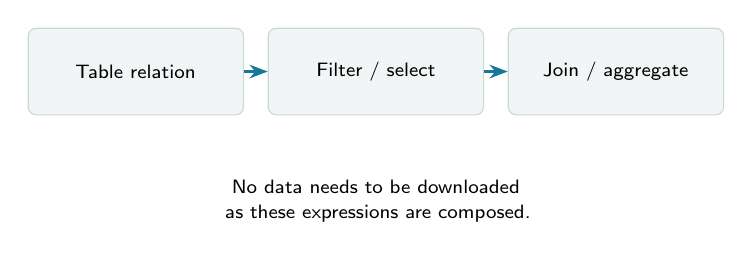
\begin{tikzpicture}[>=Stealth,every node/.style={font=\sffamily\fontsize{7.5}{9}\selectfont},n/.style={draw=thinrule,rounded corners=1mm,fill=papergray,align=center,text width=25mm,minimum height=11mm}]
\node[n](a){Table relation};\node[n,right=3mm of a](b){Filter / select};\node[n,right=3mm of b](c){Join / aggregate};
\draw[->,thick,steelblue](a)--(b);\draw[->,thick,steelblue](b)--(c);
\node[below=7mm of b,align=center,text width=65mm] {No data needs to be downloaded as these expressions are composed.};
\end{tikzpicture}\\{\fontsize{8}{9.5}\selectfont\color{inkgray}Figure 9.2. Transformations build a query plan; an action triggers execution.}\end{center}
\begin{whitebox}\textbf{Schema convention}\par
Prefer stable uppercase unquoted warehouse identifiers in the introductory lab; document exact casing and quoted-name exceptions for actual systems. Never rely on an accidental join column name or implicit cast without a schema assertion.\end{whitebox}
\repo{P097: Snowpark data engineering introductory demo}{https://github.com/Snowflake-Labs/sfguide-data-engineering-with-snowpark-python-intro}
\textbf{Check.} Why should \texttt{approved\_energy} return a DataFrame rather than call \texttt{collect()} within itself?
\newpage
% PAGE 157
\topic{9.3.2}{Lazy evaluation and action triggers}
Lazy evaluation separates the definition of a transformation from its actual evaluation. This allows a pipeline to reuse a shared filter and select only the columns required by a downstream query. It also creates a trap: a developer can mistake a constructed DataFrame for a completed side effect. For example, \texttt{session.sql('CREATE TABLE ...')} produces a DataFrame object; the command is submitted when an action such as \texttt{collect()} executes it.
\begin{lstlisting}[language=Python,caption={Actions are deliberate execution boundaries.}]
source = session.table('ENERGY_SILVER')
valid = source.filter(col('ENERGY_MWH') >= 0)
print(valid.count())              # Executes a count query
valid.limit(3).show()             # Executes and displays
rows = valid.limit(3).collect()   # Moves at most 3 rows
# valid.collect()                  # Avoid if dataset unbounded
\end{lstlisting}
\textbf{Correctness risk.} Evaluating the same lazy plan at different times can observe different committed source data. A DataFrame does not always freeze a table at the instant the Python variable is created. When a pipeline requires repeatable reconciliation, define a stable input snapshot, staging boundary or explicit temporal query. Do not compare two queries performed minutes apart and assume their source versions matched.

\textbf{Cost risk.} Three actions may run three queries, not one cached computation. A quick \texttt{count()} for a debugging message may cause a large scan. Instrument every action point and distinguish exploratory diagnostics from tasks required by the production contract.
\begin{whitebox}\textbf{Practical action checklist}\par
Before calling an action, ask: How many rows can return? Which account and warehouse executes the statement? Which source snapshot is visible? Is this an essential result or merely a debug print? Could it be replaced by a smaller deterministic assertion or an aggregate?\end{whitebox}
\textbf{Design alternative.} If a consumer only needs a total, return an aggregate DataFrame; do not collect the base data and sum it in Python. If a downstream pipeline must persist the result, use an intentional approved write path and verify its committed contents, not simply the existence of the plan object.
\repo{P098: Snowpark Python official source}{https://github.com/snowflakedb/snowpark-python}
\textbf{Check.} If a script prints the first five rows twice, what additional work might the script be requesting from Snowflake?
\newpage
% PAGE 158
\topic{9.3.3}{Inspecting execution plans and generated SQL}
A DataFrame pipeline is readable only if a reviewer can connect Python expressions to work performed by the database. Snowpark offers plan-inspection functionality, including \texttt{DataFrame.explain()} and query-generation interfaces that may vary with API release. These are \emph{diagnostics}, not guarantees of a particular optimiser plan or runtime. Use Query History and Query Profile after an authorised cloud execution to investigate actual scans, pruning and compute.
\begin{lstlisting}[language=Python,caption={Development-only plan inspection.}]
from snowflake.snowpark.functions import col
q = (session.table('ENERGY_SILVER')
     .filter(col('ENERGY_MWH') >= 0)
     .select('TECHNOLOGY', 'ENERGY_MWH'))
q.explain()  # Displays an execution-plan representation
\end{lstlisting}
Query inspection must distinguish generated SQL text from the physical execution plan selected by the service. A logical join may be reordered; a filter may be pushed down; caching may eliminate some work on a repeated query. A plan printed on an earlier API release or warehouse configuration is not a permanent contract.

For reproducible investigation, record a query tag, warehouse name and size, account edition, input row count, data profile and query ID. When comparing two plans, use the same data version and logical output. Comparing a cached aggregate against an uncached full-table export teaches little about language choice.
\begin{center}\renewcommand{\arraystretch}{1.1}\begin{tabularx}{\linewidth}{@{}p{32mm}X@{}}\toprule
\textbf{Evidence}&\textbf{What it can support}\\\midrule
Python code review&Intended filter, join and projected columns\\
Generated SQL / explain&How a DataFrame expresses a query\\
Query Profile / History&Actual operator behaviour and billed execution context\\
Output assertions&Business correctness for the tested fixture\\\bottomrule
\end{tabularx}\end{center}
\begin{insight}\textbf{Diagnostic discipline}\par
Start from the incorrect result, trace the data contract and output assertions, then inspect its physical plan when performance is the problem. Optimising a broken join can make the wrong total arrive more efficiently.\end{insight}
\repo{P099: dbt Labs Python/Snowpark Formula 1 example}{https://github.com/dbt-labs/python-snowpark-formula1}
\textbf{Check.} What evidence would distinguish a costly row export from a well-pushed-down aggregation?
\newpage
% PAGE 159
\section*{9.4\quad Transformations, joins, and aggregations}
\topic{9.4.1}{Filtering, joining, and grouping}
The energy case requires a technology-to-category lookup. A left join preserves unmatched technologies for quality review; a strict inner join could silently discard facts when a lookup value is missing. Verify that the dimension contains exactly one row per \texttt{TECHNOLOGY}, otherwise a many-to-many join can multiply MWh totals. Group only after accepted latest-state data have been selected.
\begin{lstlisting}[language=Python,caption={Core Snowpark plan used by the companion project.}]
from snowflake.snowpark.functions import col, sum as sf_sum
fact = session.table('ENERGY_SILVER')
dim  = session.table('TECHNOLOGY_DIM')
report = (fact.filter(col('OPERATION') == 'UPSERT')
         .join(dim, ['TECHNOLOGY'], 'left')
         .group_by('CATEGORY', 'INTERVAL_UTC')
         .agg(sf_sum('ENERGY_MWH').alias('TOTAL_MWH')))
\end{lstlisting}
\topic{9.4.2}{Data types and casting checks}
Treat quantity as a numeric type with suitable precision; record units explicitly. A string \texttt{'18.000'} is not automatically equivalent to a correctly validated measurement in every transformation. Use deliberate type conversion and rejection rules before an aggregate. Timestamps should represent explicit UTC source instants; local Finnish wall-clock reporting belongs in the presentation/model layer with daylight-saving behaviour specified.
\topic{9.4.3}{Validation of transformation output}
For the synthetic fixture, approved values are wind 14, solar 6, hydro 18, nuclear 16, bioenergy 8 and other 4 MWh, totalling \textbf{66.000 MWh}. Under the sample dimension, Renewable contains wind, solar, hydro and bioenergy (46 MWh); OtherLowCarbon contains nuclear (16 MWh); and Other contains the remaining 4 MWh. Those names are \emph{teaching categories}, not an official energy-sector classification.
\begin{whitebox}\textbf{Output contract}\par
Assert nonnegative measures, one current business fact per key, no unrecognised category, six visible latest-state rows, three expected category groups, and a conserved total of 66.000 MWh. A successful API call is not a passing business test.\end{whitebox}
\repo{P100: Snowpark Python demonstrations}{https://github.com/Snowflake-Labs/snowpark-python-demos}
\textbf{Check.} Which join mistake doubles the total even when every source measurement is valid?
\newpage
% PAGE 160
\section*{9.5\quad User-defined functions and stored procedures}
\topic{9.5.1}{UDFs, UDTFs, and stored procedures}
A \emph{scalar user-defined function} (UDF) returns a scalar value for its input; a \emph{user-defined table function} (UDTF) can produce multiple rows; a \emph{stored procedure} encapsulates a callable operation with control flow and, where authorised, data-management effects. These tools are useful, but not interchangeable. A built-in SQL expression should be preferred when it is sufficiently expressive, easier to optimise, and requires no bespoke Python runtime.
\begin{lstlisting}[language=Python,caption={Pure handler idea; deployment and account rights not demonstrated.}]
def normalise_label(value: str) -> str:
    return (value or '').strip().upper()
# Register as a UDF only after testing and a deployment review.
\end{lstlisting}
\topic{9.5.2}{Execution environments and appropriate use}
A Python UDF is appropriate for a deterministic, small transformation not already well supported by SQL functions. Stored procedures are better suited to multi-step application logic requiring a defined invocation and structured error reporting. A UDTF is appropriate for specialised row expansion. Consider supported runtime versions, execution permissions, scaling characteristics and the possibility that Python boundary overhead dominates a simple SQL expression.
\topic{9.5.3}{Permissions, packaging and limitations}
The deployment role may need permissions to create functions or procedures and use an internal stage for permanent handler artefacts. Installed packages must be available through supported mechanisms; an arbitrary \texttt{pip install} on a local laptop does not make a dependency available inside a managed Python handler. External network access, secrets and memory behaviour require feature-specific configuration and policy review. For regulated datasets, deliberately review whether a handler may process raw inputs.
\begin{whitebox}\textbf{Decision checklist}\par
Before registering Python code, document: output determinism; handling of nulls and exceptions; type contract; runtime/package versions; data-access and external-access permissions; test evidence; migration path; and fallback when a package version becomes unavailable.\end{whitebox}
\repo{P101: UDF and UDTF guide examples}{https://github.com/Snowflake-Labs/sfguide-UDF-UDTF-examples}
\repo{P102: External functions examples}{https://github.com/Snowflake-Labs/sfguide-external-functions-examples}
\textbf{Check.} Why is a procedure not simply a UDF with a longer Python file?
\newpage
% PAGE 161
\section*{9.6\quad Dependencies, packaging, and code organisation}
\topic{9.6.1}{Dependency pinning and compatibility}
The same notebook can behave differently months later if Snowpark or its transitive dependencies change. Keep a versioned package specification, lock exact versions before a reproducible publication release, and test against a declared Python interpreter. Constraints such as \texttt{>=1.18,<2} are a \emph{development range}, not a final reproducibility lock; the distribution of this book's eventual companion artefacts must include resolved version records.
\begin{lstlisting}[language={},caption={Project metadata; optional integrations are not installed for offline tests.}]
[project]
name = "snowflake-chapter09-energy-lab"
version = "0.1.0"
requires-python = ">=3.10"
dependencies = []
[project.optional-dependencies]
cloud = ["snowflake-snowpark-python>=1.18,<2"]
\end{lstlisting}
\topic{9.6.2}{Modular Python project layout}
Separate \emph{business rules} (version ordering, time grain, units and invalid-data policy) from \emph{connectors} (session credentials), \emph{query builders} (Snowpark DataFrames), \emph{application entry points} and \emph{tests}. Prefer functions with explicit DataFrame inputs and outputs. Avoid notebooks that rely on hidden cell order, global state or personal file paths. The companion project includes \texttt{snowpark\_pipeline.py}, \texttt{test\_snowpark.py}, \texttt{data/} fixtures and optional SQL bootstrap templates.
\topic{9.6.3}{Environment and artefact management}
Never commit credentials, downloaded personal data or run logs with secrets. Record artefact hashes where they matter, link tests to tagged source revisions, and document how to recreate the environment from a clean checkout. For deployed procedures, treat source code, package manifest and stage artefacts as a controlled release rather than an ad hoc click sequence.
\begin{insight}\textbf{Reproducibility note}\par
The printed text demonstrates a stable idea. The companion archive records the specific code and fixture used for the 22 October 2026 editorial check. A later edition should retest all feature-dependent statements and update its release tag rather than quietly changing the archive behind a printed claim.\end{insight}
\repo{P103: Snowpark on Jupyter reference}{https://github.com/Snowflake-Labs/sfguide_snowpark_on_jupyter}
\repo{P015: Snowflake Python API reference}{https://github.com/Snowflake-Labs/sfguide-snowflake-python-api}
\textbf{Check.} What additional artefact is needed to make a permissive package constraint reproducible?
\newpage
% PAGE 162
\section*{9.7\quad Local development and automated testing}
\topic{9.7.1}{Unit tests independent of live services}
Most energy-data rules can be proved without a Snowflake account: a revision must supersede an older revision, a duplicate event must not double-count, a tombstone must remove a visible fact, and a negative MWh reading must be rejected. Pure Python contract tests are fast, deterministic and free of cloud consumption. They do not establish that the Snowpark DataFrame API correctly generates the intended SQL or that account permissions are sufficient.

Snowflake also documents a \emph{local testing framework} for a subset of Snowpark DataFrame APIs. Its emulation is useful for earlier feedback but does not implement every function or exactly reproduce all warehouse behaviour. For example, the documentation distinguishes unsupported \texttt{Session.sql()} operations in local testing. Consequently, label the exact test type in the report rather than calling every successful offline test a Snowflake integration test.
\topic{9.7.2}{Integration tests in a test account}
A real integration check creates a small synthetic fixture under a disposable schema, builds the Snowpark plan and submits a deliberate action. Assert schema and numeric results, log the query ID, and remove only objects created by that test run. Repeat in the account edition and region relevant to readers if a feature varies by deployment. A test that succeeded for a six-row mock cannot prove the engine's throughput or package deployment limitations.
\topic{9.7.3}{CI secrets and expensive-test controls}
Split CI into mandatory offline tests and permission-gated cloud tests. Never enable cloud integration on every untrusted pull request, and never expose a high-privilege password to forked code. Gate paid tests behind an approval step, short-lived credentials, spending and timeout controls, and an auditable cleanup mechanism.
\begin{lstlisting}[language=bash,caption={The reproducible default is an offline test.}]
python snowpark_pipeline.py
python -m unittest -v test_snowpark.py
# Live integration: deliberately not automated by default.
\end{lstlisting}
\repo{P104: Testing Snowpark tutorial}{https://github.com/Snowflake-Labs/sftutorial-snowpark-testing}
\textbf{Check.} Which two assertions cannot be proved by an offline business-rule unit test alone?
\newpage
% PAGE 163
\section*{9.8\quad Snowpark performance and execution trade-offs}
\topic{9.8.1}{Data movement and execution locality}
A central aim of Snowpark is to let developers describe set-based work without extracting the entire dataset into a Python process. Consider two implementations of a regional generation total. Implementation A selects several million rows into pandas and groups locally. Implementation B groups by region in a Snowpark DataFrame and collects only the dozen rows of resulting totals. Both may produce correct MWh figures for a fixture; their network transfer, privacy exposure and client-memory demands are radically different.
\begin{lstlisting}[language=Python,caption={Prefer a bounded aggregate over collecting all facts.}]
from snowflake.snowpark.functions import sum as sf_sum
summary = (session.table('ENERGY_SILVER')
           .group_by('TECHNOLOGY')
           .agg(sf_sum('ENERGY_MWH').alias('MWH')))
small_result = summary.collect()  # bounded by technology count
\end{lstlisting}
\textbf{Not an unconditional guarantee.} An aggregate can still be expensive within Snowflake, especially with poor clustering, excessive cardinality or skew. The benefit is that the client receives only the result, not every source row. If grouping by an unconstrained free-text user ID, the returned result might again be huge; boundedness is a domain assertion that the test must verify.
\begin{center}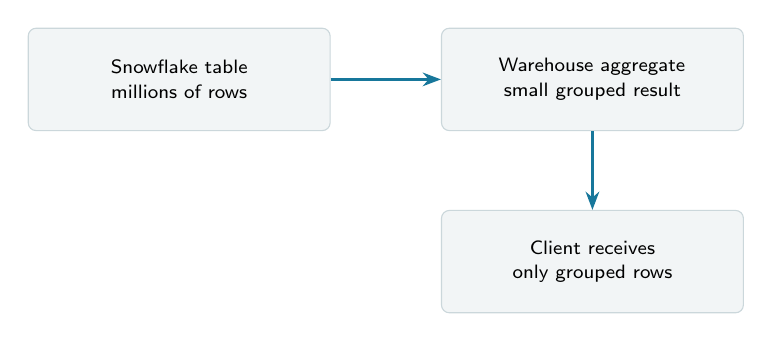
\begin{tikzpicture}[>=Stealth,every node/.style={font=\sffamily\fontsize{7.5}{9}\selectfont},n/.style={draw=thinrule,rounded corners=1mm,fill=papergray,align=center,text width=36mm,minimum height=13mm}]
\node[n](a){Snowflake table\\millions of rows};\node[n,right=14mm of a](b){Warehouse aggregate\\small grouped result};
\node[n,below=10mm of b](c){Client receives\\only grouped rows};
\draw[->,thick,steelblue](a)--(b);\draw[->,thick,steelblue](b)--(c);
\end{tikzpicture}\\{\fontsize{8}{9.5}\selectfont\color{inkgray}Figure 9.3. Push relational work to compute close to storage; transfer only necessary output.}\end{center}
\begin{whitebox}\textbf{Operational boundary}\par
Before an application collects a DataFrame, define an expected maximum number of output groups, a query timeout and a failure response. If the resulting cardinality is unexpectedly large, alert and stop rather than serialising unreviewed records to a local file.\end{whitebox}
\textbf{Check.} Which implementation exposes the larger volume of raw data outside Snowflake, and how would you prove it?
\newpage
% PAGE 164
\topic{9.8.2}{Cost and latency comparisons without misleading benchmarks}
Snowflake compute consumption depends on the services and resources actually used, not on whether an author writes \texttt{.group\_by()} or \texttt{GROUP BY}. A benchmark must control the input snapshot, output equivalence, warehouse size, concurrency and cache conditions. It must also separate client time, queueing, execution duration, data-transfer time, Python handler overhead and billed credits. Without that breakdown, a wall-clock speed comparison encourages incorrect architectural conclusions.

The energy dataset in this book is intentionally tiny: twelve synthetic deliveries and six latest-state rows. Its measured local test runtime is not meaningful evidence about production-scale warehouse latency. To compare at scale, construct an approved, suitably sized synthetic workload and publish repeatable queries, query IDs, actual credit consumption and variance across runs. A fabricated price estimate is not a benchmark.
\begin{center}\renewcommand{\arraystretch}{1.1}\begin{tabularx}{\linewidth}{@{}p{28mm}X@{}}\toprule
\textbf{Measurement}&\textbf{Required context}\\\midrule
Wall-clock latency&Start/end boundary, network, queueing, repetitions\\
Credits consumed&Warehouse and service category, idle time, time window\\
Rows scanned / output&Input version, predicates, pruning, group cardinality\\
Result correctness&Exact comparison against a reference oracle\\
Transfer volume&Bytes and number of records returned to client\\\bottomrule
\end{tabularx}\end{center}
A sound experiment might execute both SQL and Snowpark representations of the same approved hourly aggregate in a dedicated warehouse with controlled result caching. It should report \emph{median and tail durations} only after collecting real measurements. Cost optimisation then targets the observed bottleneck: fewer repeated actions, narrower scans, efficient joins, or right-sized compute. Changing languages alone is not a validated strategy.
\begin{insight}\textbf{Benchmark release rule}\par
Label every performance number as measured, simulated or illustrative. Store scripts, input generation method and raw run evidence. Never convert an unexecuted performance hypothesis into a production claim merely to make a chapter more persuasive.\end{insight}
\repo{P018: Snowpark Python performance tips}{https://github.com/Snowflake-Labs/sfguide-snowpark-python-top-three-tips-for-optimal-performance}
\textbf{Check.} Why is it invalid to compare a warm-cache aggregate with a cold-cache full export?
\newpage
% PAGE 165
\topic{9.8.3}{Avoiding Python-level anti-patterns}
Three common problems recur. \textbf{First, accidental eager collection:} an unbounded \texttt{collect()} or \texttt{to\_pandas()} pulls records into a limited client process. \textbf{Second, row-at-a-time work:} repeated queries inside a Python loop add round trips and overhead where a set-based join would suffice. \textbf{Third, unnecessary UDFs:} wrapping built-in SQL arithmetic in Python can introduce runtime and deployment cost without changing business logic.
\begin{lstlisting}[language=Python,caption={Avoid a query for every energy category.}]
# Anti-pattern (illustrative only):
# for name in thousands_of_categories:
#     session.table('ENERGY_SILVER').filter(
#         col('TECHNOLOGY') == name).collect()

# Better: one grouped relational plan.
summary = (session.table('ENERGY_SILVER')
           .group_by('TECHNOLOGY')
           .agg(sf_sum('ENERGY_MWH').alias('MWH')))
\end{lstlisting}
Optimisation does not license changing correctness requirements. If the source contains revisions, a smaller filter that discards a necessary tombstone might make a query faster while returning the wrong total. If a join's category dimension is not unique, aggregation may magnify every fact. Build tests for these risks before investigating operator-level tuning.

Another mistake is to rely on implicit ordering. Relational tables are unordered unless the query specifies an order. A preview sorted by event timestamp is a presentation choice, not a stable business resolution rule. Use explicit deterministic tie-breaking for revision events and an agreed metric grain.
\begin{whitebox}\textbf{Improve the system in this order}\par
(1) Validate the business result; (2) inspect data movement; (3) measure actual query operators; (4) reduce redundant actions; (5) tune warehouse and table design; (6) rerun correctness tests. Document any trade-off that makes the code harder to reason about.\end{whitebox}
\repo{P013: Pandas on Snowflake starting point}{https://github.com/Snowflake-Labs/sfguide-getting-started-with-pandas-on-snowflake}
\textbf{Check.} How many remote queries are issued by a loop that performs one \texttt{collect()} per source identifier?
\newpage
% PAGE 166
\section*{9.9\quad Production-oriented Python pipeline patterns}
\topic{9.9.1}{Reusable functions, configuration and logging}
Production code should separate four kinds of responsibility: connectivity, query construction, validation and publication. A \texttt{build\_report(session, ...)} function can return a lazy DataFrame. A \texttt{validate\_contract(rows)} function can run entirely offline. An orchestrator chooses when to execute and how to persist data. Each responsibility receives explicit parameters rather than importing configuration from an undocumented notebook variable.

Logs should record release version, run ID, source identifier, row-count expectations, query ID, outcome, elapsed time and object names. They should \emph{not} contain raw API secrets, passwords or unminimised personal records. A query tag can connect Snowflake Query History to a pipeline run, but it does not replace application-level data lineage or approved data retention.
\begin{lstlisting}[language=Python,caption={An original, testable function boundary.}]
def build_category_report(session, source, dimension):
    """Return a lazy, read-only DataFrame plan."""
    from snowflake.snowpark.functions import col, sum as sf_sum
    fact = session.table(source).filter(col('ENERGY_MWH') >= 0)
    dim = session.table(dimension)
    return (fact.join(dim, ['TECHNOLOGY'], 'left')
            .group_by('CATEGORY', 'INTERVAL_UTC')
            .agg(sf_sum('ENERGY_MWH').alias('TOTAL_MWH')))
\end{lstlisting}
In this abbreviated illustration, the \texttt{source} must already be latest-state, with a single approved version per business key. Production callers should use a protected table name from allowlisted configuration rather than accept unchecked SQL identifiers from external requests.
\begin{whitebox}\textbf{Logging design}\par
Persist a small JSON run ledger: input dataset version; code commit; query IDs; expected and observed row counts; aggregate checksum; error category; retry count; and final publication status. Distinguish \emph{attempt failed} from \emph{run committed}. This evidence supports both incident investigation and reader reproducibility.\end{whitebox}
\repo{P105: Snowpark DevOps reference}{https://github.com/Snowflake-Labs/snowpark-devops}
\textbf{Check.} Which elements of an execution log are essential to reproduce a faulty run without printing sensitive data?
\newpage
% PAGE 167
\topic{9.9.2}{Retries, idempotency and cleanup}
Retries are normal because transient failures occur: connections break, warehouses suspend, jobs time out and source services return errors. A retry is safe only if the intended work is idempotent or protected by an explicit transaction and publication boundary. For the energy example, replaying a previously accepted event must not create a second visible measurement. Higher revisions may change a result once; an older revision must not undo that correction.

\begin{center}\renewcommand{\arraystretch}{1.1}\begin{tabularx}{\linewidth}{@{}p{29mm}X@{}}\toprule
\textbf{Failure point}&\textbf{Safe recovery decision}\\\midrule
Before query action&Rebuild plan from versioned inputs\\
After query, before record&Check committed target / query ID; never guess\\
Partial application output&Publish through atomic or versioned boundary\\
Duplicate delivery&Deduplicate stable event ID, preserve revision order\\
Uncertain third-party effect&Use external idempotency key / reconciliation\\\bottomrule
\end{tabularx}\end{center}
A Python exception does not necessarily prove that an earlier warehouse statement rolled back. If a network connection fails after a write completes, blindly replaying the write may duplicate data. The correct response is to inspect transaction and target-state evidence and to use deterministic \texttt{MERGE} or version-based publication patterns where they fit. This is the same operational lesson as the Streams/Tasks example in Chapter~8, now expressed through a Python-controlled process.

\textbf{Cleanup should be explicit.} Temporary output artefacts may be deleted by a local test after it has preserved required assertions. Cloud objects, however, may contain other users' data or active tasks. Destructive teardown statements should remain commented until a human confirms object ownership and permissions. Never hide production cleanup inside \texttt{finally} if failure diagnostics require the data to remain for investigation.
\begin{insight}\textbf{Idempotency invariant}\par
For a fixed accepted event set, rerunning the pipeline must produce the same latest-state facts and exact MWh aggregate, regardless of repeated delivery. This is an observable property, not merely an implementation style.\end{insight}
\repo{P106: Data engineering with Snowpark Python}{https://github.com/Snowflake-Labs/sfguide-data-engineering-with-snowpark-python}
\textbf{Check.} Why is ``the Python function raised an exception'' not sufficient proof that no database changes occurred?
\newpage
% PAGE 168
\topic{9.9.3}{Monitoring, versioning and production operations}
An operational service needs signals for \emph{liveness}, \emph{freshness}, \emph{correctness} and \emph{expense}. Liveness asks whether a run finished. Freshness asks whether the latest approved interval is available within its agreed service objective. Correctness asks whether business invariants pass. Expense asks whether the observed credit and storage use remain inside a budget. A successful task status does not prove the energy aggregate is correct; conversely, a correct historical snapshot is not necessarily fresh enough for a dashboard.

\begin{whitebox}\textbf{Example monitoring contract (design targets, not measured data)}\par
Expected latest source interval: explicit UTC; max desired end-to-end freshness: 30 minutes; visible business-key duplicates: zero; rejected negative readings: quarantined and reported; aggregate reconciliation: exact for the synthetic fixture; periodic cost review: consumption by pipeline and warehouse. These thresholds are proposals that operators must approve before production use.\end{whitebox}
Release management should bind the transformation logic, fixture, dependency lock, schema definition and test output to one version identifier. Schema drift and library upgrades require an explicit compatibility test. When stored procedures are involved, account runtime and package resolution can change deployability; a successful local \texttt{pip install} is not deployment proof.

A production readiness review should also ask: What happens if the \emph{dimension table} is updated during a processing run? Can two jobs publish to the same destination at once? Is the source snapshot consistent? Are run IDs unique? Is the rollback strategy reversible? Is time-zone conversion delayed until a well-defined presentation layer? Which role owns the process when the original developer leaves?
\begin{insight}\textbf{Three questions that close the chapter}\par
Where does this Python operation actually run? How would a new engineer prove that the latest energy value is the right one? What evidence would remain after a failed or expensive run? A maintainable Snowpark design makes all three answers inspectable.\end{insight}
\textbf{Official technical references, inspected 22 October 2026:} \href{https://docs.snowflake.com/en/developer-guide/snowpark/python/working-with-dataframes}{Working with DataFrames}; \href{https://docs.snowflake.com/en/developer-guide/snowpark/python/testing-locally}{local testing framework}; \href{https://docs.snowflake.com/en/developer-guide/snowpark/python/creating-sprocs}{stored procedures}; \href{https://docs.snowflake.com/en/developer-guide/snowpark/python/creating-udfs}{Python UDFs}. Recheck version-sensitive details prior to print release.
\repo{P107: Snowpark data engineering and ML}{https://github.com/Snowflake-Labs/sfguide-getting-started-dataengineering-ml-snowpark-python}
\newpage
% PAGE 169
\section*{9.L\quad Guided lab: clean and enrich energy observations}
\topic{9.L.1}{Prerequisites, fixtures, permissions and cost guardrails}
The companion archive provides \texttt{snowpark\_pipeline.py}, \texttt{test\_snowpark.py}, \texttt{pyproject.toml}, a synthetic CSV, optional SQL bootstrap and a review worksheet. The default path uses Python~3.10+ and the standard library; it needs no account, credentials, cloud access or paid compute. Optional Snowpark DataFrame execution requires an approved Snowflake account, a limited-role warehouse and compatible package versions. No such cloud execution is claimed in this edition.

The event fixture has \textbf{12 delivered rows}, including one duplicate delivery, one superseded wind measurement, one temporary TEST reading and subsequent tombstone, plus an invalid zero revision and negative solar reading. The model enforces explicit UTC, finite nonnegative quantities, event-ID deduplication and highest revision per provider/technology/interval key. This is a \emph{synthetic} teaching dataset, not statistics from Fingrid or another external source.
\topic{9.L.2}{Step-by-step transformation and evidence}
\begin{lstlisting}[language=bash,caption={Default reproducible steps from the lab directory.}]
python snowpark_pipeline.py
python -m unittest -v test_snowpark.py
\end{lstlisting}
The first command writes three files to \texttt{output/}; the second checks twelve invariants. The Snowpark helper accepts a Session and returns an \emph{unexecuted} join-and-aggregation plan over approved source tables. It performs no write and is not imported by the offline tests.
\begin{center}\renewcommand{\arraystretch}{1.1}\begin{tabularx}{\linewidth}{@{}Xr@{}}\toprule
\textbf{Actually observed offline fixture result}&\textbf{Value}\\\midrule
Delivered rows / invalid rows&12 / 2\\
Identical event deliveries skipped&1\\
Distinct accepted valid events&9\\
Visible latest-state facts&6\\
Latest-state tombstones&1\\
Approved energy aggregate (MWh)&66.000\\
Offline unit tests passed&12 / 12\\\bottomrule
\end{tabularx}\\{\fontsize{8}{9.5}\selectfont\color{inkgray}Table 9.2. Deterministic Python result; no cloud-performance or Snowpark API test is implied.}\end{center}
\textbf{Optional integration extension:} Load exactly the six silver facts into a disposable table and a \texttt{TECHNOLOGY\_DIM} with one row per technology, then call the lazy Snowpark plan. Expect three category groups and the same 66.000 MWh after grouping. Retain query IDs and environment versions; the optional route is \emph{not executed} in this review.
\newpage
% PAGE 170
\topic{9.L.3}{Assertions, troubleshooting, rollback and cleanup}
Twelve tests verify row accounting, six approved facts, the 66.000 MWh total, wind revision precedence, tombstones, duplicate/replay handling, malformed data, revision conflicts and UTC enforcement. They prove only the tested offline Python rules, not live Snowpark execution.

If the total differs, inspect the business key and revision order. If \texttt{TEST} reappears, preserve tombstones during latest-version selection. If category totals multiply, inspect dimension uniqueness. For cloud connection errors, inspect role, warehouse and policy without exposing secrets. A local mock limitation is not evidence of an engine bug.

\textbf{Rollback and cleanup.} The default artefacts are inside \texttt{output/}; preserve evidence, then delete that local folder. No cloud teardown is active. For optional integration, approve object ownership, removal and billing evidence.
\topic{9.L.4}{Foundation, practitioner and production-design exercises}
\textbf{Foundation:} Add a duplicated wind correction with the same \texttt{EVENT\_ID}. Identify which counter changes and prove the approved total is unchanged. \textbf{Practitioner:} Add a later solar correction with a higher valid revision, then show both the new result and its invariance to replay; explain why arrival time is not the ordering key. \textbf{Production design:} Compare a single SQL model, a Snowpark DataFrame service and an external pandas service for a governed hourly dashboard. Specify data locality, role, test strategy, version pinning, latency SLO and teardown.
\begin{whitebox}\textbf{Assessment rubric (10 points)}\par
Data grain and revision semantics (2); accurate Snowpark execution-boundary explanation (2); six-row and 66.000 MWh reconciliation (2); tests and replay handling (2); cost, least privilege, evidence and cleanup (2). Full credit requires stating what was not executed.\end{whitebox}
\textbf{Chapter review.} (1) What triggers a Snowpark DataFrame action? (2) Where can Python handlers execute? (3) How would you detect an exploding join? (4) What is the difference between a local mock test and a warehouse integration test? (5) Which operational evidence should accompany a production release?

\textbf{Looking ahead.} Chapter~10 places such transformations inside dbt models and repeatable ELT delivery workflows. Python does not remove the need for declared lineage, testable contracts, or principled production releases.
\begin{insight}\textbf{Print-release verification gate}\par
Before print, recheck Snowpark runtimes and packages; execute and document a real Snowflake integration; substantiate any measured costs; and review external GitHub licensing.\end{insight}
\end{document}
